\documentclass[11pt]{article}
\usepackage{geometry}                
\geometry{letterpaper}                   

\usepackage{graphicx}
\usepackage{amssymb}
\usepackage{epstopdf}
\usepackage{natbib}
\usepackage{amssymb, amsmath}
\DeclareGraphicsRule{.tif}{png}{.png}{`convert #1 `dirname #1`/`basename #1 .tif`.png}

%\title{Title}
%\author{Name 1, Name 2}
%\date{date} 

\begin{document}



\thispagestyle{empty}

\begin{center}
\includegraphics[width=5cm]{ETHlogo.eps}

\bigskip


\bigskip


\bigskip


\LARGE{ 	Lecture with Computer Exercises:\\ }
\LARGE{ Modelling and Simulating Social Systems with MATLAB\\}

\bigskip

\bigskip

\small{Project Report}\\

\bigskip

\bigskip

\bigskip

\bigskip


\begin{tabular}{|c|}
\hline
\\
\textbf{\LARGE{Zurich traffic simulation Sihlstrasse/Uraniastrasse}}\\
\\
\hline
\end{tabular}
\bigskip

\bigskip

\bigskip

\LARGE{Filip Meier \& Sebastian Honegger}



\bigskip

\bigskip

\bigskip

\bigskip

\bigskip

\bigskip

\bigskip

\bigskip

Zurich\\
December 2015\\

\end{center}



\newpage

%%%%%%%%%%%%%%%%%%%%%%%%%%%%%%%%%%%%%%%%%%%%%%%%%

\newpage
\section*{Agreement for free-download}
\bigskip


\bigskip


\large We hereby agree to make our source code for this project freely available for download from the web pages of the SOMS chair. Furthermore, we assure that all source code is written by ourselves and is not violating any copyright restrictions.

\begin{center}

\bigskip


\bigskip


\begin{tabular}{@{}p{3.3cm}@{}p{6cm}@{}@{}p{6cm}@{}}
\begin{minipage}{3cm}

\end{minipage}
&
\begin{minipage}{6cm}
\vspace{2mm} \large Name 1

 \vspace{\baselineskip}

\end{minipage}
&
\begin{minipage}{6cm}

\large Name 2

\end{minipage}
\end{tabular}


\end{center}
\newpage

%%%%%%%%%%%%%%%%%%%%%%%%%%%%%%%%%%%%%%%



% IMPORTANT
% you MUST include the ETH declaration of originality here; it is available for download on the course website or at http://www.ethz.ch/faculty/exams/plagiarism/index_EN; it can be printed as pdf and should be filled out in handwriting


%%%%%%%%%% Table of content %%%%%%%%%%%%%%%%%

\tableofcontents

\newpage

%%%%%%%%%%%%%%%%%%%%%%%%%%%%%%%%%%%%%%%



\section{Abstract}

\section{Individual contributions}

\section{Introduction and Motivations}


The city of Zurich planing to change one specific part of the sihlstrasse in a pedestrian area. The idea is to make this area more comfortable for the visitors of the city center and it should be also an upgrade for the restaurants and shops around this area.
\begin{figure}[h]
\begin{minipage}[t]{.45\textwidth}
	\centering
	\vspace{30pt}
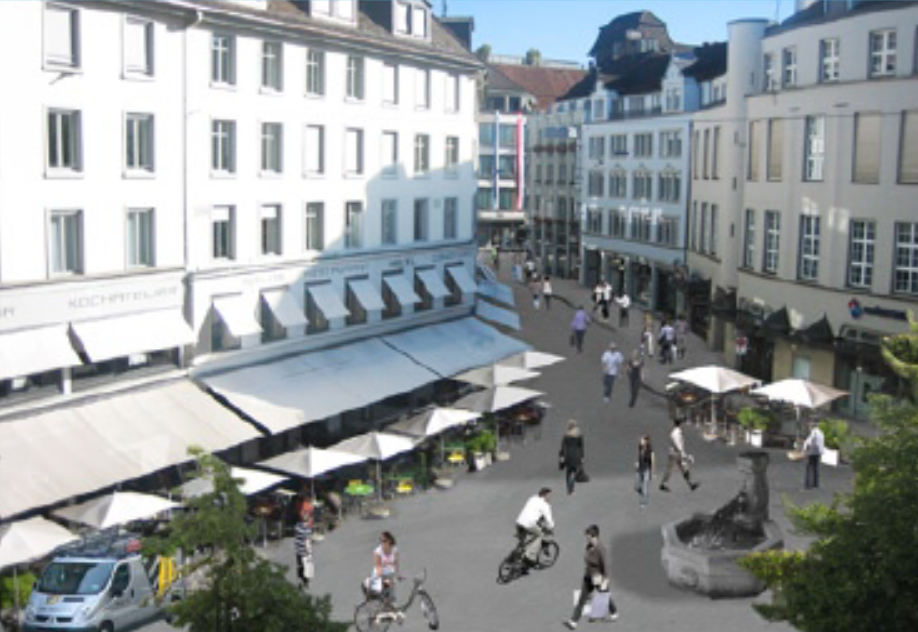
\includegraphics[width=\textwidth]{pedestrianarea.png}
\end{minipage}\hfill
\begin{minipage}[t]{.45\textwidth}
	\centering
	\vspace{0pt}
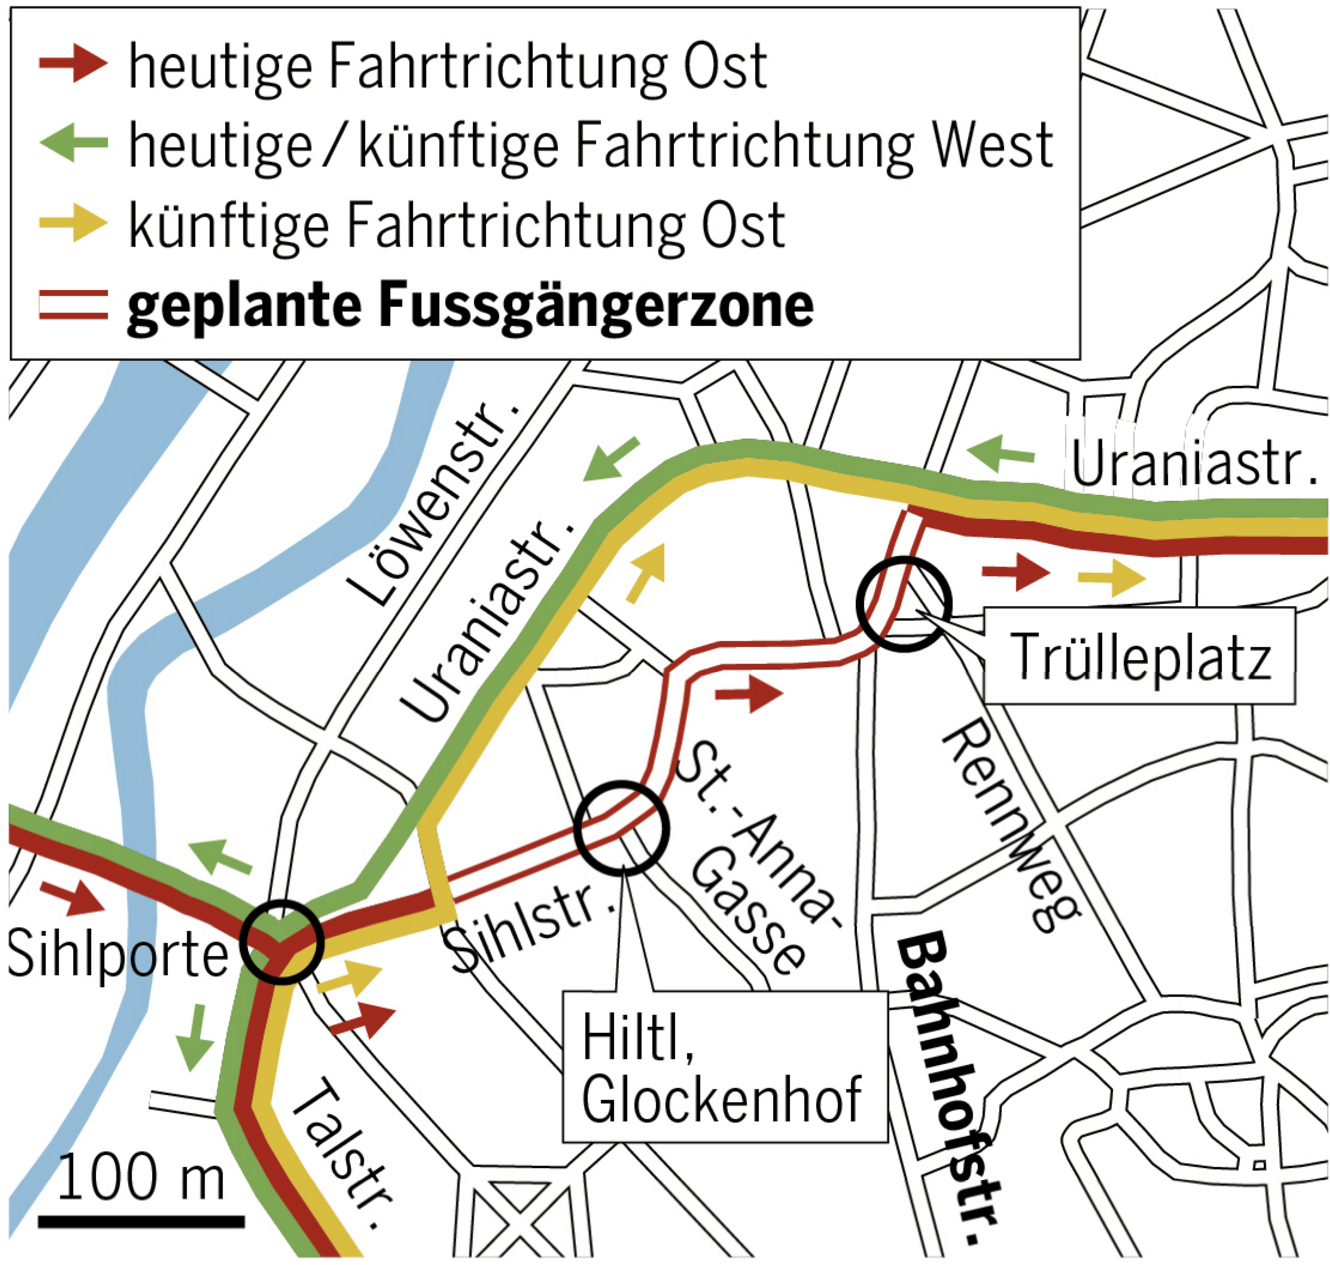
\includegraphics[width=\textwidth]{Plan_Sihlstrasse.png}
\end{minipage}\hfill
\caption{right: situation plan which shows the change of the tracks. left: illustraion of the pedestrian area at sihlstrasse.}
\end{figure}
\\
The changet will have a big impact for the traffic because there will be one track less than before. Sihlstrasse (from west to east) and Uraniastrasse (from east to west) is one of the most travelled  road in the city center. It is the only alternative road to the highway (Westumfarung). If they decide to built a pedestrian area in the sihlstrasse they will lose one track from west to east.
We know want to analyse the impact to the traffic jam and the impact on the neighbourhood streets.

\section{Fundamental Questions}

With our simulation, we want to answered the following questions:
\begin{itemize}
\item[1.] Are the streets still large enough to manage the traffic jam peaks on working days?
\item[2.] What is the impact on the neigbourhood streets?
\item[3.] Which area or signal light is the bottleneck?
\end{itemize}
\section{Description of the Model}

\subsection{Nagel-Schreckenberg-model}

Our model is based on the prototype of cellular automata model which is called \textit{Nagel-Schreckenber-model}. It was developed by Kai Nagel and Michael Schreckenberg in 1992. The basic idea was to split the streets in cells, which contain only one car. Therefore we can identify on cell with the typical required space for one car in a traffic jam. Generally this length is around $7.5\,\mathrm{m}$, which correspond approximately the length of the car and the average distance to the car in front in a traffic jam.
\begin{figure}[h!]
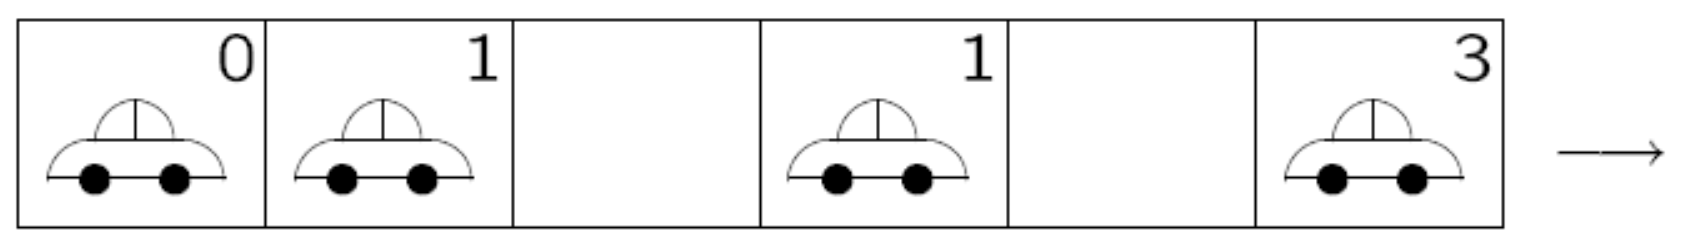
\includegraphics[width=\textwidth]{ns_config.png}
\caption{this figure illustrate the typical \textit{Nagel-Schreckenberg-model} configuration: one cell (approx. $7.5\,\mathrm{m}$) which can include exactly one car.}
\label{ns_config} 
\end{figure}
Figure (\ref{ns_config}) shows a typical \textit{Nagel-Schreckenberg-model} set-up, one cell (approx. $7.5\,\mathrm{m}$) which include one car. The number in the upper right corner of the cell (which include a car) representing the actual velocity $v_n$ of the car $n$. The velocity is a discrete value an we assume that the car $n$ can have the velocities $v_n=0,1 \ldots ,v_{\mathrm{max}}$. Every car has the same $v_{\mathrm{max}}$ which has the same effect like a speed limit.\\
With this properties one have a good description of the state of the street at time $t$. The next step is to define the development in time. So we have to define the state of the street at the time $t+1$. To simulate this time step in the \textit{Nagel-Schreckenberg-model} we have to define for steps, which we have to apply for each car $n$:
\begin{itemize}
\item[1.]	\textbf{Acceleration}\\
\\
If $v_n<v_{\mathrm{max}}$ at time $t$, the car $n$ will accelerate is velocity about one unit:
\begin{equation}
v_n \rightarrow v'_n = \min(v_n+1,v_\mathrm{max})
\label{accel}
\end{equation}
$v'_n$ represents the new velocity at time $t+1$.
\item[2.]  \textbf{Slow down}\\
\\
We define $d_n$ as the number of empty cells in front of the car $n$ until to the next car $n+1$. So if $d_n$ is smaller than $v'_n$, the car $n$ has to slow down to the velocity $d_n$:
\begin{equation}
v'_n \rightarrow v''_n = \min(v_n',d_n)
\label{slowd}
\end{equation}
\item[3.]  \textbf{Hang behind}\\
\\
If $v''_n>0$, the velocity of car $n$ will be randomly with the probability $p$ reduced about one unit:
\begin{equation}
v''_n \rightarrow v'''_n=
\begin{cases}
\max(v''_n-1,0) & \mathrm{with\,probability} \quad p\\
v''_n & \mathrm{with\,probability} \quad 1-p
\end{cases}
\label{hangb}
\end{equation}
\item[4.] \textbf{Drive}\\
\\
The car $n$ drives with the new velocity $v_n(t+1)=v'''_n$ about $v_n(t+1)$ cells:
\begin{equation}
x_n(t+1)=x_n(t)+v_n(t+1)
\label{drive}
\end{equation}
\end{itemize}
One have to apply every step simultaneous to every car. So we can not simulate the real situation, that the car in front can move as well simultaneous to the car behind.
\\
One can see that just step (\ref{slowd}) has a interaction between cars and with step (\ref{hangb}) the simulations has a stochastic  dynamic. Therefore the \textit{Nagel-Schreckenberg-model} is called a stochastic cellular automata.
\\
\begin{figure}[h!]
\begin{itemize}
\item[1.] \textbf{start configuration} \\
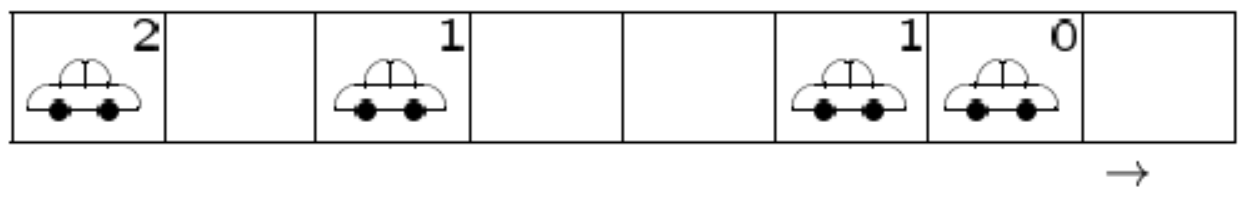
\includegraphics[width=\textwidth]{config_1.png}
\item[2.] \textbf{acceleration} ($v_{\mathrm{max}}=2$) \\
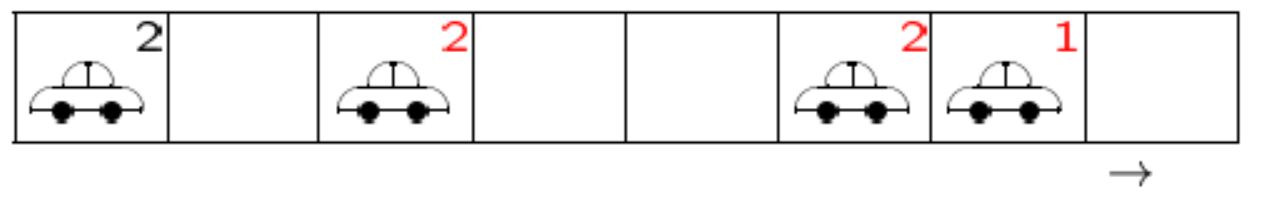
\includegraphics[width=\textwidth]{config_2.png}
\item[3.] \textbf{slow down} \\
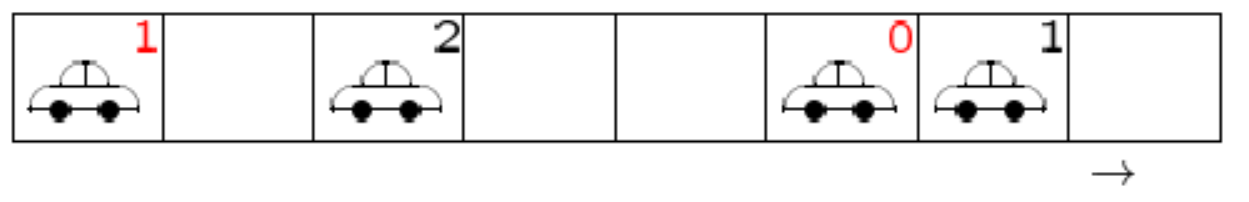
\includegraphics[width=\textwidth]{config_3.png}
\item[4.] \textbf{hang behind} ($p=\frac{1}{3}$) \\
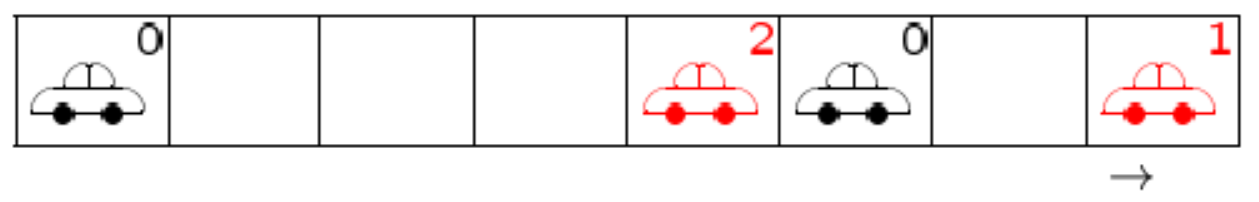
\includegraphics[width=\textwidth]{config_4.png}
\item[4.] \textbf{drive} ($=$ configuration at $t+1$) \\
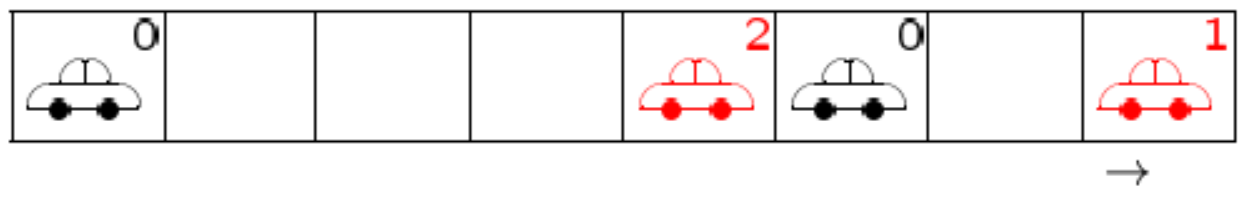
\includegraphics[width=\textwidth]{config_5.png}
\end{itemize}
\caption{Shows on complete time step of the \textit{Nagel-Schreckenberg-model} with acceleration, slow down, hang behind probability and drive.}
\label{example_ns} 
\end{figure}
Figure (\ref{example_ns}) shows a complete time step of the \textit{Nagel-Schreckenberg-model}. In this case in step 4 we have three car which are able to hang behind but just one will to it in the next step (probability $p=\frac{1}{3}$). And as one can see the speed limit in this example is $v_\mathrm{max}=2$.
\begin{itemize}
\item[1.] The first step in figure \ref{example_ns} shows that all cars want to accelerate as soon as possible to maximum speed limit.
\item[2.] the 'slow down' step (figure \ref{example_ns} prevent car accidents. But as mention before it does not include the movement of the car in front at the same time.
\item[3.] The step hang behind simulates different effects. It tries to modelling for example natural fluctuations in driving style. A normal car drives never with a total constant speed it always fluctuate between $v_\mathrm{max}$ und $v_\mathrm{max}-1$. This function generates an asymmetry for the acceleration and the slow down mode. In detail it will generate a stronger slow down and sometimes the speed stays constant instead to accelerate. If we have a high density of cars, the above described effects could have a traffic jam as result.
\item[4.] The last step is just the motion of the cars with the new speed which is compute with the steps 1 to 3.

\end{itemize}

We already defined the length of one cell ($7.5\,\mathrm{m}$) but we also have to define the correct time scale fpr one time step $t$ $\rightarrow$ $t+1$. Therefore we need a value for the average speed, one can calculate it in the following way:\\

\begin{equation}
v_\mathrm{aver}=(1-p)v_\mathrm{max} + p(v_\mathrm{max}-1)=v_\mathrm{max}-p
\label{average_speed}
\end{equation}
We now identify this speed with $50\,\mathrm{km/h}$. For a model with $v_\mathrm{max}=5$ and $p=0.5$ we get\\
\begin{equation}
\frac{7.5\,\mathrm{m}}{\mathrm{cells}}\cdot\frac{4.5\,\mathrm{cells}}{\mathrm{timestep}} \cdot \frac{3.6\,\mathrm{s}}{50\,\mathrm{m}}\approx 2.5\,\frac{\mathrm{s}}{\mathrm{timestep}}
\end{equation}

\subsection{Chowdhury-Schadschneider-Modell}

The dynamic of a real city traffic is characterized through the interaction of two time scales, the driving time between two traffic lights and the time of the green phase of each traffic light. Chowdhury and Schadschneider have modify the \textit{Nagel-Schreckenberg-model} with a algorithm for traffic lights to simulate the traffic of a city. The dynamic is define by the following steps. $d_n$ define as before the gap to the next car and $s_n$ defines the distance to the next traffic light:\\

\begin{itemize}
\item[1.]	\textbf{Acceleration}\\
\\
If $v_n<v_{\mathrm{max}}$ at time $t$, the car $n$ will accelerate is velocity about one unit:
\begin{equation}
v_n \rightarrow v'_n = \min(v_n+1,v_\mathrm{max})
\label{accel_t}
\end{equation}
$v'_n$ represents the new velocity at time $t+1$.
\item[2.]  \textbf{Slow down because of cars or traffic lights}\\
\\
\begin{itemize}
\item[1.]case: The traffic light is red:
\begin{equation}
v'_n \rightarrow \min(v_n,d_n,s_n)
\end{equation}
\item[2.]case: The traffic light is green:
\begin{itemize}
\item[a.] The traffic light get red in the next time step:
\begin{equation}
v'_n \rightarrow \min(v_n,d_n,s_n)
\end{equation}
\item[b.] The traffic light is not getting red:
\begin{equation}
v'_n \rightarrow \min(v_n,d_n)
\end{equation}
\end{itemize}

\end{itemize}
\item[3.]  \textbf{Hang behind}\\
\\
If $v''_n>0$, the velocity of car $n$ will be randomly with the probability $p$ reduced about one unit:
\begin{equation}
v''_n \rightarrow v'''_n=
\begin{cases}
\max(v''_n-1,0) & \mathrm{with\,probability} \quad p\\
v''_n & \mathrm{with\,probability} \quad 1-p
\end{cases}
\label{hangb}
\end{equation}
\item[4.] \textbf{Drive}\\
\\
The car $n$ drives with the new velocity $v_n(t+1)=v'''_n$ about $v_n(t+1)$ cells:
\begin{equation}
x_n(t+1)=x_n(t)+v_n(t+1)
\label{drive}
\end{equation}
\end{itemize}
The simulations is exactly like the \textit{Nagel-Schreckenberg-model} just the interaction with the traffic lights in step 2 is new. If we have a red traffic light the has to stop before. Therefore the velocity $v_n$ of car $n$ should not be higher then the distance $s_n$ to the next traffic light. So the car will be affected by the traffic light if $s_n<v_n$.\\
If the traffic light is green we can simulate a kind of orange phase. If the traffic light gets red in the next step, the cars will slow down immediately. If the traffic light not get red the simulation will just look on the distance to the next car.

\section{Implementation}

\section{Simulation Results and Discussion}

\section{Summary and Outlook}

\section{References}






\end{document}  



 
